\documentclass{article}

\usepackage{amsmath,amssymb}
\usepackage{mathrsfs}
\usepackage{tensor}
\usepackage{fullpage}

\usepackage{graphicx}

\usepackage{textpos}
\usepackage{eso-pic}
\usepackage{tikz}
\usetikzlibrary{tikzmark}

\title{Noether's Theorem}
\author{Anthony Mezzacappa}
\date{September 15 and 17, 2020}
% Typeset by Wileam Phan
% Diagram in Page 2a by Wileam Phan

\begin{document}

\setlength{\parskip}{1em}

\maketitle

\noindent If $\phi$ satisfies the Euler-Lagrange EOM ($\delta S = 0$), for \underline{any} variation we have
\begin{equation*}
    \delta \mathscr{L} = \partial_\mu \left( \dfrac{ \partial \mathscr{L} }{ \partial ( \partial_\mu \phi ) } \delta \phi \right) \tikzmarknode{deltaL}{}
\end{equation*}

{%
\begin{textblock*}{3in}(4in,-1.4in)%
\begin{minipage}[h!]{3in}
    \small%
    \begin{center}
        \boxed{REMINDER}
    \end{center}
    \vspace*{-12pt} \begin{align*}
        \tikzmarknode{inset}{~} \delta \mathscr{L} &= \bigg[ \overbrace{ \dfrac{ \partial \mathscr{L} }{ \partial \phi } - \partial_\mu \left( \dfrac{ \partial \mathscr{L} }{ \partial ( \partial_\mu \phi ) } \right) }^{=0} \bigg] \delta \phi \\
        &\quad + \partial_\mu \left( \dfrac{ \partial \mathscr{L} }{ \partial ( \partial_\mu \phi ) } \delta \phi \right) \\
        &= \partial_\mu \left( \quad \right) \\
        \delta S &= \int \mathrm{d}^4 x~ \delta \mathscr{L} \\
        &= \int \mathrm{d}^4 x~ \partial_\mu ( \quad ) \\
        &= 0
    \end{align*}
\end{minipage}%
\end{textblock*}%
}%
\begin{tikzpicture}[overlay, remember picture]
    \draw[overlay,->] (inset.north) -- (deltaL.west);
\end{tikzpicture}

\vspace*{-24pt} \noindent Assume the action also has the symmetry
\begin{equation*}
    \delta_\Delta S = 0
\end{equation*}
under the \underline{specific} transformation
\begin{equation*}
    \phi \longrightarrow \phi + \Delta
\end{equation*}

\noindent Given the action is invariant under the transformation even though the \linebreak Lagrangian density may not be,
\begin{equation} \label{l8a-eq1}
    \delta_\Delta \mathscr{L} = \partial_\mu \left( \dfrac{ \partial \mathscr{L} }{ \partial ( \partial_\mu \phi ) } \Delta \right) \neq 0
\end{equation} % Equation 1
\begin{equation} \label{l8a-eq2}
    \delta_\Delta \mathscr{L} = \partial_\mu \tensor{K}{^\mu}
\end{equation} % Equation 2
\begin{equation*}
    \delta_\Delta S = \int \mathrm{d}^4 x~ \delta_\Delta \mathscr{L} = \int \mathrm{d}^4 x~ \partial_\mu \tensor{K}{^\mu} = 0
\end{equation*}
-- i.e., $\delta_\Delta \mathscr{L}$ must be a total divergence. Equating \eqref{l8a-eq1} and \eqref{l8a-eq2}, we get
\begin{equation*}
    \partial_\mu \left( \dfrac{ \partial \mathscr{L} }{ \partial ( \partial_\mu \phi ) } \Delta - \tensor{K}{^\mu} \right) = 0
\end{equation*}
-- i.e., we have a \underline{conserved current} ($\partial_\mu \tensor{j}{^\mu} = 0$)
\begin{equation*}
    \tensor{j}{^\mu} \equiv \dfrac{ \partial \mathscr{L} }{ \partial ( \partial_\mu \phi ) } \Delta - \tensor{K}{^\mu}
\end{equation*}
so, with a symmetry there is a conserved current.


% Page 1a

\noindent A conserved current will be associated with a conserved "charge"
\begin{equation*}
    \partial_\mu \tensor{j}{^\mu} = \partial_0 \tensor{j}{^0} + \partial_i \tensor{j}{^i}
\end{equation*}

\noindent Integrate over all of space
\begin{equation*}
    \int \mathrm{d}^3 x~ \left( \partial_0 \tensor{j}{^0} + \partial_i \tensor{j}{^i} \right) = 0
\end{equation*}

\noindent Then
\begin{align*}
    \partial_0 \int \mathrm{d}^3 x~ \tensor{j}{^0} &= - \int \mathrm{d}^3 x~ \partial_i \tensor{j}{^i} \\
    &= 0
\end{align*}
and we identify
\begin{equation*}
    Q \equiv \int \mathrm{d}^3 x~ \tensor{j}{^0}
\end{equation*}
with the conserved "charge".

% Page 2a

\noindent\rule{\textwidth}{.5pt}

\noindent Consider a coordinate transformation corresponding to a spacetime translation
\begin{equation*}
    \mathbf{x} \longrightarrow \mathbf{x}' = \mathbf{x} - \mathbf{a}
\end{equation*}
.i.e.,
\begin{equation*}
    \tensor{x}{^\mu} \longrightarrow \tensor{x}{^\prime^\mu} = \tensor{x}{^\mu} - \tensor{a}{^\mu}
\end{equation*}
where
\begin{equation*}
    \tensor{a}{^\mu} = ( \tensor{a}{^0}, \tensor{a}{^1}, \tensor{a}{^2}, \tensor{a}{^3} )
\end{equation*}
and $\tensor{a}{^0^,^1^,^2^,^3}$ are all constants (they can be different).

\noindent Consider three points $P$, $Q$, and $R$, and their coordinates before and after the transformation:
\begin{figure}[h!]
    \centering
    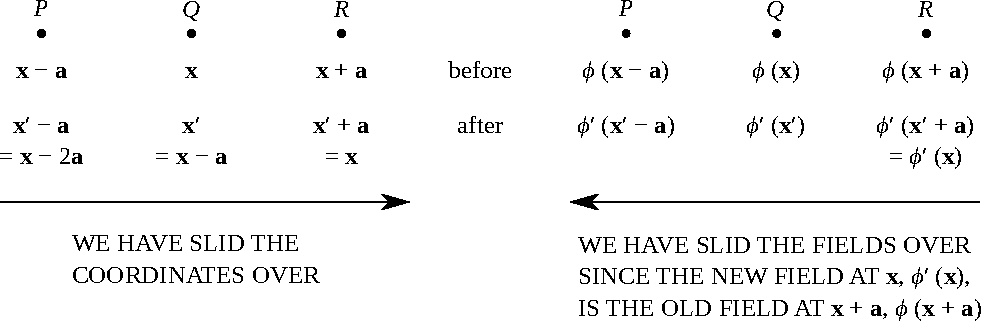
\includegraphics[width=.99\textwidth]{pics/07-coordinate-transformation.pdf} %
    \label{fig:l7-coordinate-transformation}
\end{figure}

\newpage

\noindent So, \underline{at $\mathbf{x}$}, \underline{we have replaced} the field \underline{$\phi (\mathbf{x})$ by $\phi ( \mathbf{x} + \mathbf{a} )$}, and
\begin{align*}
    \delta \phi (\mathbf{x}) &= \phi' (\mathbf{x}) - \phi (\mathbf{x}) \\
    &= \phi ( \mathbf{x} + \mathbf{a} ) - \phi (\mathbf{x}) \\
    &= \phi (\mathbf{x}) + \tensor{\partial}{_\mu} \phi (\mathbf{x}) \tensor{a}{^\mu} - \phi (\mathbf{x}) \\
    &= \tensor{\partial}{_\mu} \phi (\mathbf{x}) \tensor{a}{^\mu}
\end{align*}

\noindent It is in the sense that we mean we have moved the fields rather than the coordinates, which is a viewpoint that emerges when we focus \underline{on a given $\mathbf{x}$}.

\noindent This is the ACTIVE viewpoint.

\noindent The PASSIVE viewpoint emerges when we focus on what happens \underline{at a specific} \underline{point} (e.g., $Q$):

\vspace*{-16pt} \begin{center}
\begin{tabular}{lcc}
    at $Q$: & $\phi' (\mathbf{x}') = \phi (\mathbf{x})$ & $\phi' (Q) = \phi(Q)$ \\
    at $R$: & $\phi' ( \mathbf{x}' + \mathbf{a} ) = \phi ( \mathbf{x} + \mathbf{a} )$ & $\phi' (R) = \phi (R)$
\end{tabular}
\end{center} \vspace*{-16pt}

\noindent i.e., the \underline{\underline{value}} of the scalar field at a point does not change as the coordinates of the point change
\begin{equation*}
    \delta \phi (Q) = \phi' (\mathbf{x}') - \phi (\mathbf{x}) = 0
\end{equation*}

\noindent\rule{\textwidth}{.5pt}

% Page 2

\noindent How do we find $\tensor{K}{^\mu}$?

\noindent Consider the \underline{translation invariance} of the action under the transformation
\begin{equation*} % Note: tensor package doesn't like \tensor{x'}{^\mu}
    \tensor{x}{^\mu} \longrightarrow \tensor{x}{^\prime^\mu} = \tensor{x}{^\mu} - \tensor{a}{^\mu}
\end{equation*}

\noindent Then
\begin{equation*}
    \phi (\mathbf{x}) \longrightarrow \phi ( \mathbf{x} + \mathbf{a} ) = \phi (\mathbf{x}) + \dfrac{ \partial \phi }{ \partial \tensor{x}{^\mu} } \tensor{a}{^\mu}
\end{equation*}
and
\begin{equation*}
    \delta_\Delta \phi = \dfrac{ \partial \phi }{ \partial \tensor{x}{^\mu} } \tensor{a}{^\mu}
\end{equation*}

\noindent Then
\begin{align*}
    \delta_\Delta \left( \tensor{\partial}{_\mu} \phi \right) &= \tensor{\partial}{_\mu} \left( \delta_\Delta \phi \right) \\
    &= \tensor{\partial}{_\mu} \! \left( \dfrac{ \partial \phi }{ \partial \tensor{x}{^\alpha} } \tensor{a}{^\alpha} \right) \\
    &= \dfrac{ \partial^2 \phi }{ \partial \tensor{x}{^\mu} \tensor{x}{^\alpha} } \tensor{a}{^\alpha}
\end{align*}

\noindent Now we can compute
\begin{align*}
    \delta_\Delta \mathscr{L} &= \dfrac{ \partial \mathscr{L} }{ \partial \phi } \delta_\Delta \phi + \dfrac{ \partial \mathscr{L} }{ \partial ( \tensor{\partial}{_\mu} \phi ) } \delta_\Delta ( \tensor{\partial}{_\mu} \phi ) \\
    &= \dfrac{ \partial \mathscr{L} }{ \partial \phi } \dfrac{ \partial \phi }{ \partial \tensor{x}{^\alpha} } \tensor{a}{^\alpha} + \dfrac{ \partial \mathscr{L} }{ \partial ( \tensor{\partial}{_\mu} \phi ) } \dfrac{ \partial^2 \phi }{ \partial \tensor{x}{^\mu} \tensor{x}{^\alpha} } \tensor{a}{^\alpha} \\
    &= \left( \dfrac{ \partial \mathscr{L} }{ \partial \phi } \dfrac{ \partial \phi }{ \partial \tensor{x}{^\alpha} } + \dfrac{ \partial \mathscr{L} }{ \partial ( \tensor{\partial}{_\mu} \phi ) } \dfrac{\partial}{ \partial \tensor{x}{^\alpha} } \! ( \tensor{\partial}{_\mu} \phi ) \right) \tensor{a}{^\alpha} \\
    &= \dfrac{ \partial \mathscr{L} }{ \partial \tensor{x}{^\alpha} } \tensor{a}{^\alpha} \\
    &= \tensor{\partial}{_\alpha} ( \mathscr{L} \tensor{a}{^\alpha} )
\end{align*}

% Page 3

\noindent Then
\begin{equation*}
    \tensor{K}{^\mu} = \mathscr{L} \tensor{a}{^\mu}
\end{equation*}
and
\begin{align*}
    \tensor{j}{^\mu} &= \dfrac{ \partial \mathscr{L} }{ \partial ( \tensor{\partial}{_\mu} \phi ) } \Delta - \tensor{K}{^\mu} \\
    &= \dfrac{ \partial \mathscr{L} }{ \partial ( \tensor{\partial}{_\mu} \phi ) } \dfrac{ \partial \phi }{ \partial \tensor{x}{^\alpha} } \tensor{a}{^\alpha} - \mathscr{L} \tensor{a}{^\mu} \\
    &= \left( \dfrac{ \partial \mathscr{L} }{ \partial ( \tensor{\partial}{_\mu} \phi ) } \dfrac{ \partial \phi }{ \partial \tensor{x}{^\alpha} } - \mathscr{L} \tensor{\delta}{^\mu_\alpha} \right) \tensor{a}{^\alpha}
\end{align*}

\noindent Then
\begin{equation*}
    \tensor{\partial}{_\mu} \tensor{j}{^\mu} = \tensor{a}{^\alpha} \tensor{\partial}{_\mu} \left( \dfrac{ \partial \mathscr{L} }{ \partial ( \tensor{\partial}{_\mu} \phi ) } \dfrac{ \partial \phi }{ \partial \tensor{x}{^\alpha} } - \mathscr{L} \tensor{\delta}{^\mu_\alpha} \right) = 0
\end{equation*}

\noindent Since $\tensor{a}{^\alpha}$ is arbitrary, for the above to be true always, each "coefficient" of $\tensor{a}{^\alpha}$ must be zero:
\begin{equation*}
    \tensor{\partial}{_\mu} \left( \dfrac{ \partial \mathscr{L} }{ \partial ( \tensor{\partial}{_\mu} \phi ) } \dfrac{ \partial \phi }{ \partial \tensor{x}{^\alpha} } - \mathscr{L} \tensor{\delta}{^\mu_\alpha} \right) = 0
\end{equation*}

\noindent Contract with $\tensor{\eta}{^\nu^\alpha}$
\begin{equation*}
    \tensor{\partial}{_\mu} \left( \underbrace{ \dfrac{ \partial \mathscr{L} }{ \partial ( \tensor{\partial}{_\mu} \phi ) } \dfrac{ \partial \phi }{ \partial \tensor{x}{_\nu} } - \mathscr{L} \tensor{\eta}{^\mu^\nu} } \right) = 0
\end{equation*}
\begin{equation*}
    = \tensor{T}{^\mu^\nu}
\end{equation*}

{%
\begin{textblock*}{2in}(3in,-1.25in)%
\begin{minipage}[h!]{2in}
    \begin{align*}
        &\longleftarrow \tensor{\eta}{^\nu^\alpha} \tensor{\partial}{_\mu} (\qquad) = 0 \\
        &\qquad \Rightarrow \tensor{\partial}{_\mu} [ \tensor{\eta}{^\nu^\alpha} (\qquad) ] = 0
    \end{align*}
\end{minipage}%
\end{textblock*}%
}
{%
\begin{textblock*}{2in}(2.7in,-0.2in)%
\begin{minipage}[h!]{2in}
    \noindent The energy-momentum tensor for the scalar field $\phi$
\end{minipage}%
\end{textblock*}%
}

% Page 3a

\newpage

\begin{equation*}
    \tensor{\partial}{_\mu} \tensor{T}{^\mu^\nu} = 0
\end{equation*}

\begin{equation*}
    \tensor{\partial}{_0} \tensor{T}{^0^\nu} + \tensor{\partial}{_i} \tensor{T}{^i^\nu} = 0
\end{equation*}

\noindent \underline{$\nu = 0$}
\begin{equation*}
    \tensor{\partial}{_0} \tensor{T}{^0^0} + \tensor{\partial}{_i} \tensor{T}{^i^0} = 0 \hspace{0.5in} \mathrm{conservation} ~ \mathrm{of} ~ \mathrm{energy}
\end{equation*}
\begin{equation*}
    \tensor{\partial}{_0} \int \mathrm{d}^3 x~ \tensor{T}{^0^0} = \tensor{\partial}{_0} \int \mathrm{d}^3 x~ \mathscr{H} = - \int \mathrm{d}^3 x~ \tensor{\partial}{_i} \tensor{T}{^i^0}
\end{equation*}
$\Rightarrow H = \int \mathrm{d}^3 x~ \mathscr{H}$ is the conserved "charge"

\noindent \underline{$\nu = j$}
\begin{equation*}
    \tensor{\partial}{_0} \tensor{T}{^0^j} + \tensor{\partial}{_i} \tensor{T}{^i^j} = 0 \hspace{0.5in} \mathrm{conservation} ~ \mathrm{of} ~ \mathrm{momentum}
\end{equation*}
\begin{equation*}
    \tensor{\partial}{_0} \int \mathrm{d}^3 x~ \tensor{T}{^0^j} =  - \int \mathrm{d}^3 x~ \tensor{\partial}{_i} \underbrace{ \tensor{T}{^i^j} } = 0
\end{equation*}
\hspace*{2.7in} {\small stress tensor}

$\Rightarrow \tensor{P}{^i} = \int \mathrm{d}^3 x~ \underbrace{ \tensor{T}{^0^i} }$ is the conserved "charge"
\\ \hspace*{0.75in} {\small momentum density}

\noindent\rule{\textwidth}{.5pt}

% Page 4

\noindent What about Lorentz invariance?

\begin{equation*}
    \tensor{x}{^\beta} \longrightarrow \tensor{\Lambda}{^\beta _\nu} \tensor{x}{^\nu} = \tensor{x}{^\beta} - \underbrace{ \tensor{\varepsilon}{^\beta _\nu} \tensor{x}{^\nu} }_{ \equiv \delta \tensor{x}{^\beta} } = \tensor{x}{^\beta} - \delta \tensor{x}{^\beta}
\end{equation*}

\noindent\rule{\textwidth}{.5pt}

\noindent For the case where there is relative motion in the $x$-direction only, we know that the $(t, x)$ and $(t', x')$ coordinates are related by
\begin{align*}
    t' &= \gamma ( t - \beta x ) \\
    x' &= \gamma ( x - \beta t )
\end{align*}
where
\begin{align*}
    \gamma &= {[ 1 - \left( \dfrac{v}{c} \right) ]}^{ -\frac{1}{2} } \\
    \beta &= \dfrac{v}{c}
\end{align*}
and $v$ is the relative velocity.

\noindent Then
\begin{equation*}
    \tensor{x}{^\prime^\mu} = %
    \begin{pmatrix}
        t' \\
        x' \\
        y' \\
        z'
    \end{pmatrix}%
    = %
    \begin{pmatrix}
        \gamma & - \gamma \beta & 0 & 0 \\
        - \gamma \beta & \gamma & 0 & 0 \\
        0 & 0 & 0 & 0 \\
        0 & 0 & 0 & 0
    \end{pmatrix}%
    \begin{pmatrix}
        t \\
        x \\
        y \\
        z
    \end{pmatrix}%
    \equiv \tensor{\Lambda}{^\mu _\nu} \tensor{x}{^\nu}
\end{equation*}

\noindent\rule{\textwidth}{.5pt}

% Back to Page 4

\noindent Then
\begin{equation*}
    \phi (\mathbf{x}) \longrightarrow \phi ( \Lambda^{-1} \mathbf{x} ) \tikzmarknode{lambda}{=} \phi (\mathbf{x}) - \dfrac{ \partial \phi }{ \partial \tensor{x}{^\alpha} } \delta \tensor{x}{^\alpha}
\end{equation*}
and
\begin{align*}
    \delta_\Delta \phi &= \dfrac{ \partial \phi }{ \partial \tensor{x}{^\alpha} } \delta \tensor{x}{^\alpha} \\
    &= \tensor{\partial}{_\alpha} \phi ~ \tensor{\varepsilon}{^\alpha _\nu} \tensor{x}{^\nu}
\end{align*}

\noindent Then
\begin{align*}
    \delta_\Delta ( \tensor{\partial}{_\mu} \phi ) &= \tensor{\partial}{_\mu} ( \delta_\Delta \phi ) \\
    &= \tensor{\partial}{_\mu} \left( \tensor{\partial}{_\alpha} \phi ~ \tensor{\epsilon}{^\alpha _\nu} \tensor{x}{^\nu} \right) \\
    &= ( \tensor{\partial}{_\mu} \tensor{\partial}{_\alpha} \phi ) ~ \tensor{\epsilon}{^\alpha _\nu} \tensor{x}{^\nu} + \tensor{\partial}{_\alpha} \phi ~ \tensor{\varepsilon}{^\alpha _\nu} \tensor{\delta}{^\nu _\mu} \\
    &= ( \tensor{\partial}{_\mu} \tensor{\partial}{_\alpha} \phi ) ~ \tensor{\varepsilon}{^\alpha _\nu} \tensor{x}{^\nu} + \tensor{\partial}{_\alpha} \phi ~ \tensor{\varepsilon}{^\alpha _\mu}
\end{align*}

\noindent Now
\begin{align*}
    \delta_\Delta \mathscr{L} &= \dfrac{ \partial \mathscr{L} }{ \partial \phi } ~ \delta_\Delta \phi + \dfrac{ \partial \mathscr{L} }{ \partial ( \tensor{\partial}{_\mu} \phi ) } ~ \delta_\Delta ( \tensor{\partial}{_\mu} \phi ) \\
    &= \dfrac{ \partial \mathscr{L} }{ \partial \phi } ~ \tensor{\partial}{_\alpha} \phi ~ \tensor{\varepsilon}{^\alpha _\nu} \tensor{x}{^\nu} + \dfrac{ \partial \mathscr{L} }{ \partial ( \tensor{\partial}{_\mu} \phi ) } \left[ ( \tensor{\partial}{_\mu} \tensor{\partial}{_\alpha} \phi ) ~ \tensor{\varepsilon}{^\alpha _\nu} \tensor{x}{^\nu} + \tensor{\partial}{_\alpha} \phi ~ \tensor{\varepsilon}{^\alpha _\mu} \right] \\
    &= \dfrac{ \partial \mathscr{L} }{ \partial \tensor{x}{^\alpha} } ~ \tensor{\varepsilon}{^\alpha _\nu} \tensor{x}{^\nu} + \dfrac{ \partial \mathscr{L} }{ \partial ( \tensor{\partial}{_\mu} \phi ) } ~ \tensor{\partial}{_\alpha} \phi ~ \tensor{\varepsilon}{^\alpha _\mu}
\end{align*}

% Page 5


\end{document}